% IFAC International Federation of Automatic Control paper template. 
% Created by: ?
% Modified by: Rasmus Christensen, Aalborg University, Denmark 15/12/2012
\documentclass{ifacconf}

\usepackage{natbib}            % you should have natbib.sty
\usepackage{graphicx}          % Include this line if your 
                               % document contains figures,
%\usepackage[dvips]{epsfig}    % or this line, depending on which
                               % you prefer.
\usepackage[utf8]{inputenc} % So we can input Nicks name in the paper title!
\usepackage[T1]{fontenc}
\usepackage{amsmath,amsfonts,amssymb} % Added so we can do pretty math equations.

% predefined environments
%\begin{thm} ... \end{thm}		% Theorem
%\begin{lem} ... \end{lem}		% Lemma
%\begin{claim} ... \end{claim}	% Claim
%\begin{conj} ... \end{conj}	% Conjecture
%\begin{cor} ... \end{cor}		% Corollary
%\begin{fact} ... \end{fact}	% Fact
%\begin{hypo} ... \end{hypo}	% Hypothesis
%\begin{prop} ... \end{prop}	% Proposition
%\begin{crit} ... \end{crit}	% Criterion


\begin{document}

\begin{frontmatter}

\title{Centralized State Estimation of Distributed Maritime Autonomous Surface Oceanographers\thanksref{footnoteinfo}} % Title, preferably not more than 10 words.

\thanks[footnoteinfo]{Thanks to the  has been paid for in full by the School of Information Communication and Technology.}

\author[First]{Rasmus L. Christensen} 
\author[First]{Frederik Juul} 
\author[First]{Nick \O stergaard}
\author[First]{Attila Fodor}
\author[First]{Tudor Muresan}
\address[First]{Department of Electronic Systems, Aalborg University, Fredrik Bajers Vej 7, 9220 Aalborg \O st, Denmark (e-mail: \{ralch,nickoe,fjuul,tudor,attila\}@es.aau.dk)}                                            
          
\begin{keyword}                           % Five to ten keywords,  
Path planning; Centralised control; Baud rates; State estimation; Marine systems; Master slave system;              % chosen from the IFAC 
\end{keyword}                             % keyword list or with the 
                                          % help of the Automatica 
                                          % keyword wizard


\begin{abstract}                          % Abstract of not more than 250 words.
This paper considers the subject of running a centralized controller for the purpose of navigating a small Autonomous Surface Vehicle (ASV). The centralized controller is using a Kalman filter as a state predictor to improve the precision of the navigational aids mounted aboard. The work presents the design of the motion control system as well as the development of a protocol used to push through as much data on a standard 9.6 kbps data link simplex link.

The performance for the algorithms developed in this project, have been tested in Limfjorden in Aalborg, and towards the end, results of these tests are shown. 
\end{abstract}

\end{frontmatter}

\section{Introduction}
As up to date mapping of the coastal areas around Greenland is not available, and the process of creating these are a both time consuming and expensive task. One way to reduce both the costs and the amount of time invested in such a project could be to develop small autonomous drones to carry out this task. 

These drones should be controlled by a mothership, which would utilize a simple data link, both to preserve bandwith, but also to make the duration at which the ships are able to sail as long as possible, by limiting the power consumption. 

Currently the main focus of autonomous vehicles have been on aerial, ground and underwater vehicles, why there is close to no research going on about small autonomous surface vessels. An example of such a vessel is the Stingray ASV developed by Isreali Based Elbit Systems. The purpose of this vehicle is somewhat military related, where the purpose of measuring the coastal areas around Greenland are purely humanitarian,

{\bf Do not change the font sizes or line spacing to squeeze more text into a limited number of pages. Use italics for emphasis; do not underline}.

\subsection{Problem statement}
\begin{hypo} Is it possible to develop a centralized state estimator for use in the maritime environment using a small data link \end{hypo}

\subsection{A subsection}

\begin{figure}
	\begin{center}
		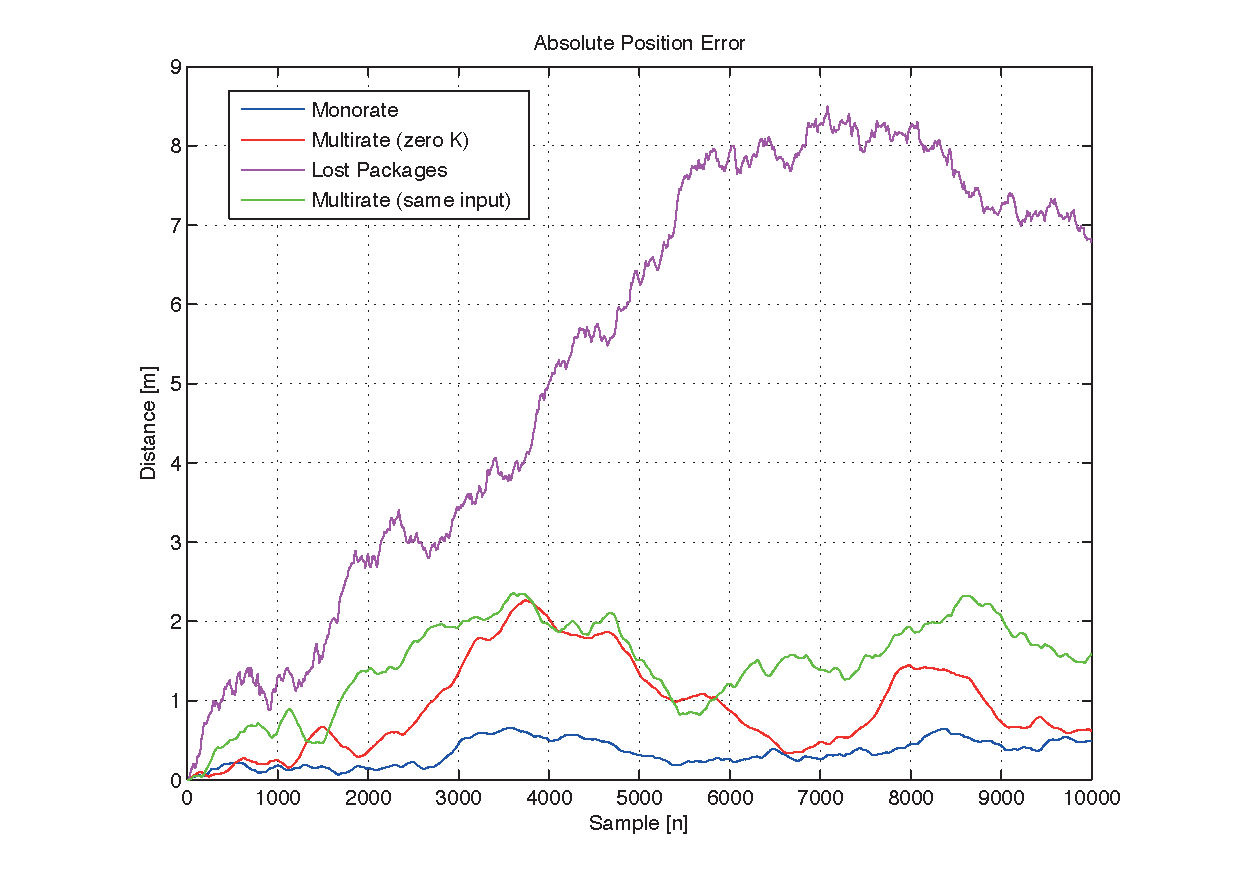
\includegraphics[width=8.4cm]{img/10percent} % width of a column is 8.4 cm.
		\caption{Bifurcation: Plot of local maxima of $x$ with damping $a$ decreasing}  
		\label{fig:fig1}
	\end{center}
\end{figure}

\section{Methods}

The methods developed in this project - and the papers. 2

\subsection{Path planning algorithm}

The path planning algorithm is based around the train-track transition problem originally stated by SOMEBODY, which divides the path into straight and turning parts and describes the transition between these using the normalized Fresnel integral, describing an Euler spiral, which allows the ship to maintain a linear acceleration through the turn, thus keeping the amount of jerk $j$ as close to zero as possible. The two Fresnel integrals are given as in equation (\ref{eq:fresnel}):
\begin{align}
C_F(x) = \int_0^x \cos(t^2)dt,\,\,\,\,S_F(x) = \int_0^x \sin(t^2)dt
\label{eq:fresnel}
\end{align}
When two normalized Fresnel integrals are plotted simultaniously they produce the Euler spiral. However, the benefit of using such a spiral is only present if the angle of the incoming ship is larger than some threshold $\varepsilon$. If $\varepsilon$ is smaller than the threshold, the path can be approximated by a smooth curve, which is computationally easier to handle, thus saving time before the control signals are sent back. Figure (\ref{fig:3points}) depicts how the system computes and places the sub-waypoints for when $\varepsilon$ is below $\varepsilon_{max}$, as this approximation only uses the curvature of a circle, only 3 sub-waypoints are generated. 
\begin{figure}
	\begin{center}
		\includegraphics[width=8.4cm]{img/3points} % width of a column is 8.4 cm.
		\caption{Path planning when $\varepsilon$ < $\varepsilon_{max}$, the path is approximated by a curve and only 3 sub-waypoints are generated, denoted $A_3$, $C_3$ and $E_3$}
		\label{fig:3points}
	\end{center}
\end{figure}
The 3 sub-waypoints are given by the coordinate sets:
\begin{align}
A_3 = (-X_1,Y_1),\, C_3 = (0,\frac{y_d}{cos(\varepsilon)}),\, E_3 = (X_1,Y_1)
\end{align}
From where the individual coordinates can be computed by simple trigonometric equations. As the coordinates are mirrored around $x=0$ the it is only required to do 2 coordinate computations - given as:
\begin{align}
X_1 = x_d(\varepsilon) \cdot \cos(\varepsilon) + y_d(\varepsilon) \cdot \sin(\varepsilon),\,\,\, Y_1 = X_1 \cdot 	\tan(\varepsilon)
\end{align}
Where $x_d(\varepsilon)$ and $y_d(\varepsilon)$ is the normalized Fresnel integral function of the angle $\varepsilon$ at which the ship is approaching the turn thus:
\begin{align}
x_d = \frac{\pi}{\eta}\cdot C_F(\varepsilon),\,\,\, y_d = \frac{\pi}{\eta}\cdot S_F(\varepsilon),\,\,\, \eta = \frac{\text{max}\{\dot{\alpha}\}}{v^2}
\end{align}
Once the angle grows larger than $\varepsilon_{max}$ the system has to compute extra sub-waypoints, as the ship must transit onto a curve, and then back onto a straight line once done turning. This adds the extra waypoints $B_5$ and $D_5$, as well as the circle around which the ship is turning. This circle has centre in $O_5$ and a radius of $R_{min}$. The waypoints are depicted on figure (\ref{fig:5points}), thus augmenting the waypoints to:
\begin{figure}
	\begin{center}
		\includegraphics[width=8.4cm]{img/5points}    % The printed column  
		\caption{Path planning when $\varepsilon$ < $\varepsilon_{max}$, the path is approximated by a curve and only 3 sub-waypoints are generated, denoted $A_5$, $B_5$, $C_5$, $D_5$ and $E_5$}  % width of a column is 8.4 cm.
		\label{fig:3points}               
	\end{center}                                 % accordingly.
\end{figure}
\begin{align}
A_5 &= (-X_1,Y_1),\, B_5 = (-X_2,Y_2),\, C_5 = (0,Y_R)\\
D_5 &= (X_2,Y_2),\, E_5 = (X_1,Y_1)
\end{align}
Which is still a mirroring of points about the $x=0$ axis, as the entry angle is the same as the exit angle. The number of equations increases, and the individual coordinates can be computed by:
\begin{align}
X_R &= R_\text{min} \cdot \sin(\varepsilon - \varepsilon _\text{max})\\
P_X &= X_R + y_d \cdot \sin(\varepsilon)\\
X_1 &= P_X + x_d \cdot \cos(\varepsilon)\\ 
Y_1 &= X_1 \cdot \tan(\varepsilon)\\
P_Y &= Y_1 - x_d \cdot \sin(\varepsilon)\\
Y_2 &= P_Y + y_d \cdot \cos(\varepsilon)\\
O_Y &= R_\text{min} \cdot \cos(\varepsilon - \varepsilon _\text{max}) + Y_2\\
R_Y &= O_Y - R_\text{min}\\
X_2 &= X_R
\end{align}
The above equations conclude the development of the path planner. Other than that it generates straight lines on which the ship is to run.

Using a threshold to determine wether the turn can be made using just a circle approximation, or a transition onto a circle is needed (if the turn is too sharp). 

\subsection{State estimation}
To give a better estimate of position and the attitude of the craft, a Kalman filter have been implemented to improve the accuracy of the sensors mounted aboard the ship. To develop a such, the discrete time state model of the ship have been derived to be:
\begin{align}
\vec{\Phi} = diag\{\vec{\Phi} _x,\vec{\Phi} _y,\vec{\Phi} _\omega\}
\end{align}
Where the diagonal entries $\vec{\Phi} _x,\vec{\Phi} _y,\vec{\Phi} _\omega$ are given by the same equation, with different entries:
\begin{align}
\vec{\Phi}_{x,y,\omega}(k) = \begin{bmatrix}
1 & t_s & 0\\
0 & 1 & t_s\\
0 & \frac{-\beta_{x,y,\omega}}{m,m,I} & 0
\end{bmatrix}
\end{align}
Where $\beta_{x,y,\omega}$ denotes the skin frictional drag in the $x$,$y$ or $\omega$ direction respectively, $m$ is the mass of the craft, $I$ is the interia and $t_s$ is the sampling time of the filter. The states to be estimated for the controller are:
\begin{align}
^b\hat{\vec{x}_k} = \begin{bmatrix}
x & \dot{x} & y & \dot{y} & \theta & \omega
\end{bmatrix}^T
\end{align}
The observation model of the filter does however contain more measurements, and the measurements can be given as:
\begin{align}
\vec{v}_k = \begin{bmatrix}
x & \dot{x} & \ddot{x} & y & \dot{y} & \ddot{y} & \theta & \omega
\end{bmatrix}^T
\end{align}
The implementation of the filter is an altered version of an Linear Minimum Mean Square Error filter - the alteration lies in the Kalman gain, where a matrix mask $\Lambda$ is post multiplied. This matrix mask is to zero out the measurements that are invalid. This matrix mask is defined as:
\begin{align}
\\vec{\Lambda} = diag\{\lambda_x,\lambda_{\dot{x}},\lambda_{\ddot{x}},\lambda_{\lambda{y}},\lambda_{\dot{y}},\lambda_{\ddot{y}},\lambda_{\theta},\lambda_{\omega},\lambda_{\alpha} \}
\end{align}
This ensures that when a measurement is invalid (the checksum is not true) the receiver zeros out the gain, and runs the filter on the other sensors / estimates. 
As all the forces are acting on the ship in the inertial body fixed frame - the 

\section{Math}
Some mathematics go here. 

\section{Units}

\section{Results}

\subsection{Model of the ship}
The model of the ASV is in continuos time given as the state space equation defined in (eq:\ref{eq:ss_cont}) - the model considers the motion of the ship with 3 degrees of freedom, movement in the x-direction, y-direction and rotation about the z-axis. 
\begin{align}
\dot{\begin{bmatrix}
v\\
\theta\\
\omega
\end{bmatrix}} = \begin{bmatrix}
\frac{-\beta_v}{m} & 0 & 0\\
0 & 0 & 1\\
0 & 0 & \frac{-\beta_\omega}{I}
\end{bmatrix} + \begin{bmatrix}
\frac{1}{m} & 0\\
0 & 0\\
0 & \frac{1}{I}
\end{bmatrix}
\label{eq:ss_cont}
\end{align}
This model is sufficient as it is only the velocity and the angle that is desired to cont as the other states are uncontrollable by the ship in its current configuration. The control strategy is to track the input reference, and use an optimal feedback gain to reach the desired values. This is done as in REFERENCE! giving the following gains:
\begin{align}
F_opt &= \\
N &= 
\end{align}
The above might be stupid to include? 

\subsection{Control verification}
Running the system with just the controllers produces the following plot trying to follow a path around the parking lot. 

\subsection{Path planning results}
Planning the path on a stretch of water in Aalborg produces the following results:

\subsection{Kalman filtering verification}
Filtering the above traced controller route with the Kalman filter, having the input to the system to zero, and post processing the data produces the following plot.

\subsection{Combined test}
Running the Kalman filter on the ship whilst in motion. As seen some packages are lost - to verify the simulator, a simulation have been run with the same amount of packages lost, and this produces the same result. 

Something about the packet loss. 

\subsection{Other tests}

Something else?


\section{Conclusion}

A conclusion section is not required. Although a conclusion may review the main points of the paper, do not replicate the abstract as the conclusion. A conclusion might elaborate on the importance of the work or suggest applications and extensions. 

\begin{ack}                               % Place acknowledgements
A special thank should be given to Assistant Professor Carles Navarro Manch�n, Section for Navigation and Communication, Department of Electronic Systems, Aalborg University for his help with tuning the Kalman filter.  % here.
\end{ack}

%\bibliographystyle{alpha}        % Include this if you use bibtex 
%\bibliography{autosam}           % and a bib file to produce the 
%\bibliography{autosam}
                                 % bibliography (preferred). The
                                 % correct style is generated by
                                 % Elsevier at the time of printing.

\begin{thebibliography}{xx}

\bibitem[Able(1956)]{Abl:56}
B.C. Able.
\newblock Nucleic acid content of microscope.
\newblock \emph{Nature}, 135:\penalty0 7--9, 1956.

\bibitem[Able et~al.(1954)Able, Tagg, and Rush]{AbTaRu:54}
B.C. Able, R.A. Tagg, and M.~Rush.
\newblock Enzyme-catalyzed cellular transanimations.
\newblock In A.F. Round, editor, \emph{Advances in Enzymology}, volume~2, pages
  125--247. Academic Press, New York, 3rd edition, 1954.

\bibitem[Keohane(1958)]{Keo:58}
R.~Keohane.
\newblock \emph{Power and Interdependence: World Politics in Transitions}.
\newblock Little, Brown \& Co., Boston, 1958.

\bibitem[Powers(1985)]{Pow:85}
T.~Powers.
\newblock Is there a way out?
\newblock \emph{Harpers}, pages 35--47, June 1985.

\bibitem[Soukhanov(1992)]{Heritage:92}
A.~H. Soukhanov, editor.
\newblock \emph{{The American Heritage. Dictionary of the American Language}}.
\newblock Houghton Mifflin Company, 1992.

\end{thebibliography}








\appendix
\section{A summary of Latin grammar}    % Each appendix must have a short title.
\section{Some Latin vocabulary}         % Sections and subsections are supported  
                                        % in the appendices.
\end{document}